% Metódy inžinierskej práce

\documentclass[10pt,twoside,slovak,a4paper]{article}

\usepackage[slovak]{babel}
\usepackage[T1]{fontenc}
\usepackage[IL2]{fontenc} 
\usepackage[utf8]{inputenc}
\usepackage{graphicx}
\usepackage{url} 
\usepackage{hyperref} 

\usepackage{cite}
\usepackage{times}

\pagestyle{headings}

\title{Vývoj zvukových kodekov\thanks{Finálna verzia článku semestrálneho projektu v predmete Metódy inžinierskej práce, ak. rok 2021/22, vedenie: Vladimír Mlynarovič}} 

\author{Hlib Kokin\\[2pt]
	{\small Slovenská technická univerzita v Bratislave}\\
	{\small Fakulta informatiky a informačných technológií}\\
	{\small \texttt{xkokin@stuba.sk}}
	}

\date{\small 12. decembra 2021} 



\begin{document}

\maketitle

\begin{abstract}
Tento článok bude hovoriť o zvukových kodekoch. 
Článok sa  začiná všeobecnými pojmami o zvukových kodekoch a ich histórii v prvej časti, potom si povie o základoch stratového kódovania zvuku(v časti čislo dva) a v ďalšej časti budú informácie o princípoch zvuku bluetooth. Ďalej  v článku bude analýza rozdielov medzi AUX a Bluetooth a na záver vám článok povie o možných spôsoboch vývoja kodekov v budúcnosti. 
\end{abstract}
\newpage
\section{Pokrok vyvoja kodekov} \label{pokrok}

Táto časť článku bude hovoriť o základných pojmoch o kodekoch, histórii ich vývoja v prvej kapitole, zmienime o kodekoch, ktoré sú dnes populárne v v ďalšej kapitole.

"Codec" je skratka pre encode/decode. Môžu byť hardvérové alebo softvérové – obe prijímajú analógový signál a konvertujú ho do digitálneho formátu. Funkcia dekódovania je presne ten istý proces, ale obrátený, aby sa digitálny dátový tok mohol previesť na analógové zvukové vlny na výstup.\cite{Stephens}

Diagram \ref{f:rozhod1} ukazuje, na aké typy sa zvukové kodeky delia.
\begin{figure*}[tbh]
\centering
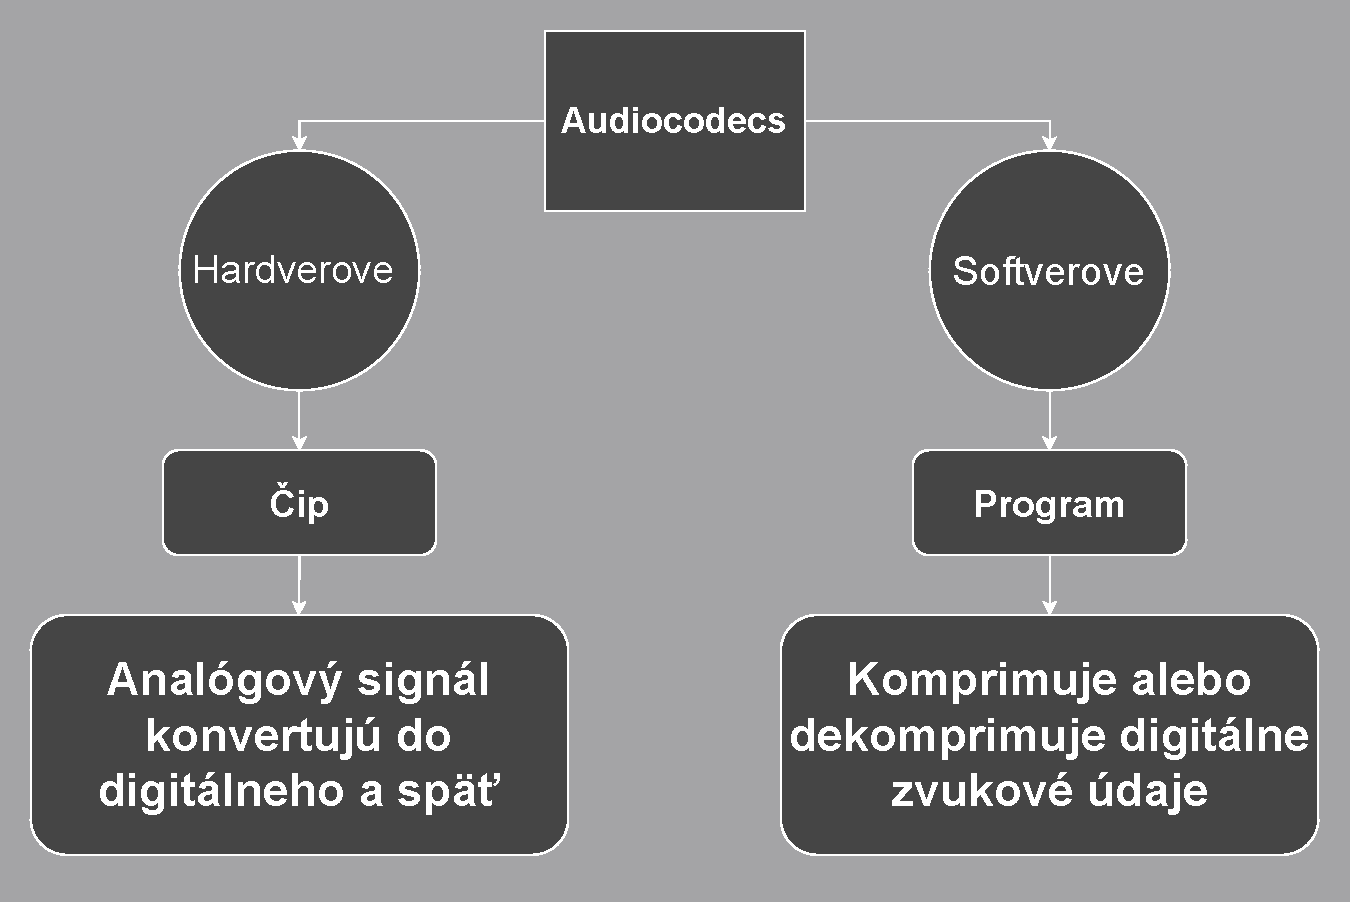
\includegraphics[scale=0.5]{Typy_kodekov.pdf}
\caption{Typy kodekov.}
\label{f:rozhod1}
\end{figure*}

Existujú tri kategórie kodekov: nekomprimovaný, stratový a bezstratový a podrobné vysvetlenie o nich bude popísané v časti~\ref{stratové kódovanie}.

\subsection{História kodekov} \label{história} 

Od prvého známeho zvukového záznamu v roku 1860 na fonautografe sa technológia záznamu a prehrávania zvuku neustále mení. 20. storočie prinieslo éru profesionálnych zvukových nahrávačov a inžinierov, vek prenosu zvuku cez rádiové vlny, obrovský pokrok v kvalite a technológii zvuku a pokračujúci rast v audio priemysle – a obchode vo všeobecnosti. \cite{Stephens} 

V roku 1982 urobil svet zvuku prvé kroky do nového tisícročia s vôbec prvým digitálnym audio formátom – kompaktným diskom. CD, postavené na prelomovej technológii Pulse Code Modulation (PCM), dokázalo uložiť analógové zvukové vlny ako digitálne hodnoty ich „kvantovaním“ na ich najbližšiu podporovanú digitálnu hodnotu.\cite{Stephens} 

Obrázok \ref{f:rozhod0} schematicky ukazuje, ako funguje modulácia pulzného kódu  
\begin{figure*}[tbh]
\centering
\includegraphics[scale=0.5]{Pcm.png}
\caption{Pulse Code Modulation (PCM).\cite{Stephens} }
\label{f:rozhod0}
\end{figure*}

Modulácia pulzného kódu odštartovala novú éru inovácií pre digitálne audio formáty. V priebehu desiatich rokov si známe moderné kodeky ako MP3 a WAV získavali trakciu. Začiatkom roku 2000 došlo k prvej vlne bezstratových zvukových kodekov, ktoré priniesli digitálnu kvalitu ešte vyššie bez kompromisov veľkých veľkostí súborov.\cite{Stephens}

Ale tieto vynikajúce formáty neboli pripravené na šialenstvo MP3 prehrávačov zo začiatku tisícročia. iPod od Apple priviedol masy do sveta digitálneho zvuku a MP3 sa stal celosvetovým štandardom pre prehrávanie zvuku.\cite{Stephens}

\subsection{Dnešné kodeky}  \label{populárne kodeky}  

V súčasnosti sa v mnohých odvetviach používa veľa zvukových kodekov. Mnoho záznamov v tomto zozname bolo predstavených pred desaťročiami, existuje však niekoľko nových kodekov, ktoré osvetľujú potenciál, ktorý budúcnosť zvukových kodekov ponúka. 

Tabuľka \ref{f:rozhod3} zobrazuje päť populárnych kodekov a ich charakteristiky. 
\begin{figure*}[tbh]
\centering
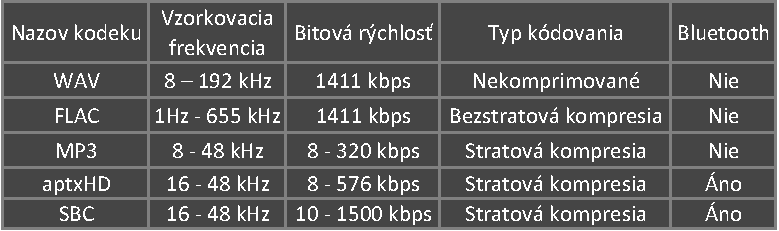
\includegraphics[scale=1.0]{porovnanie_kodekov.pdf}
\caption{Porovnanie kodekov.\cite{Logvinov, ValdikSS}}
\label{f:rozhod3}
\end{figure*}

\section{Základy stratového kódovania zvuku.} \label{stratové kódovanie}

Táto časť začne informáciami o bezstratovom a bezkompresnom kódovaní. Ďalej sa pozrime na princípy stratových kodekov a bezstratových

Diagram \ref{f:rozhod2} ukazuje typy kódovania a prenosu signálu. 
\begin{figure*}[tbh]
\centering
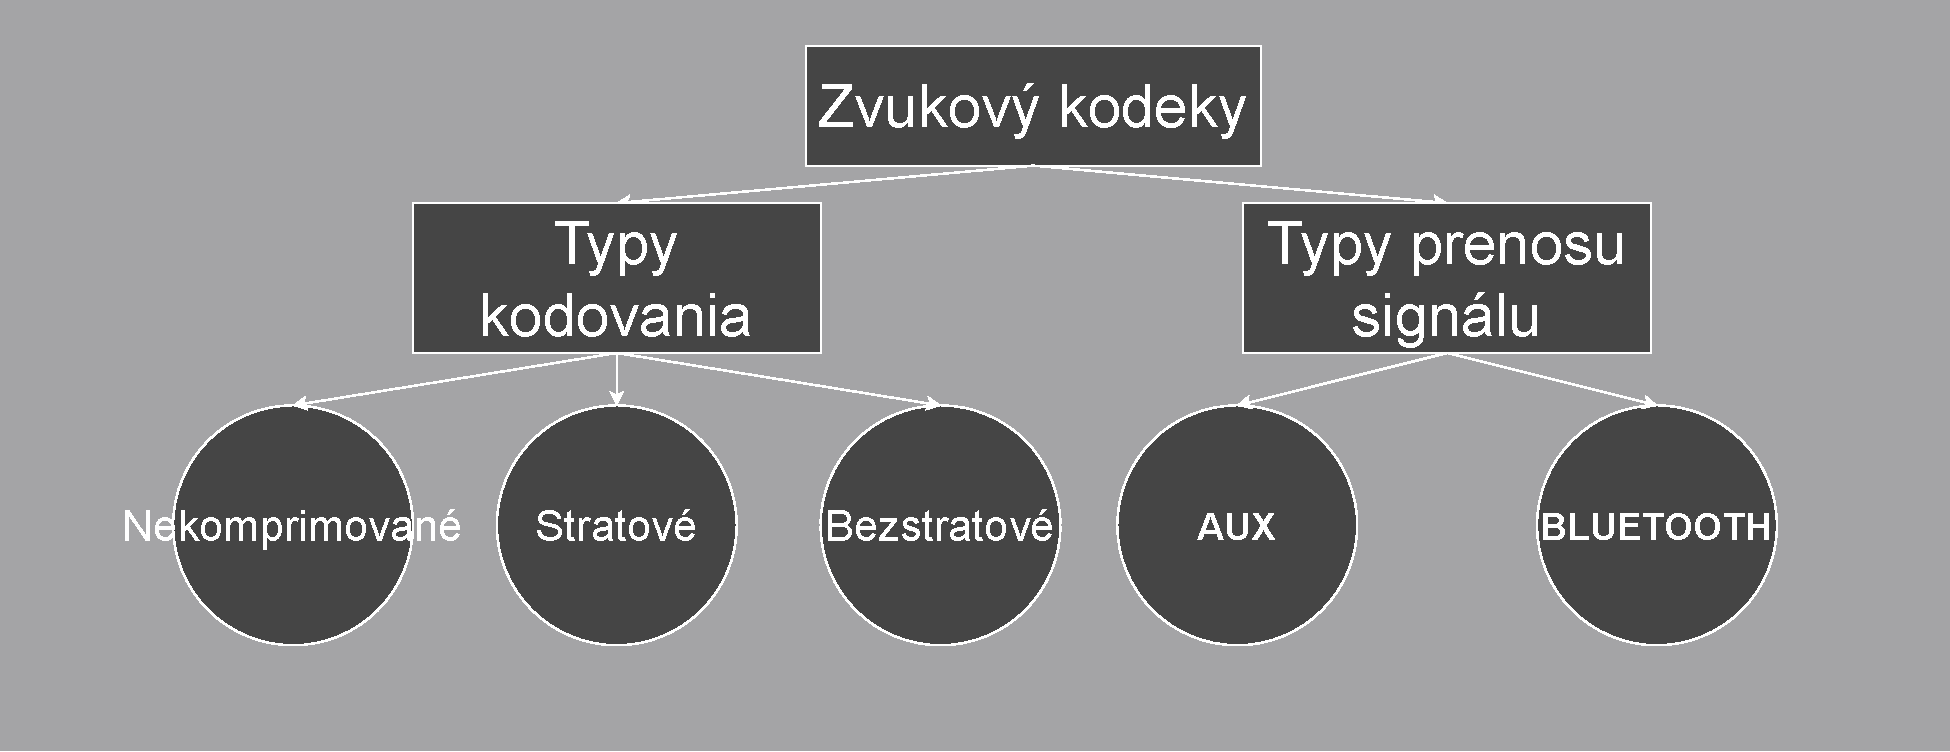
\includegraphics[scale=0.4]{Typy_kodovania_prenosu.pdf}
\caption{Typy kódovania a prenosu signálu.}
\label{f:rozhod2}
\end{figure*}

\paragraph{Nekomprimované kódovanie} \label{nekomprimované} \cite{Logvinov}

Nekomprimované zvukové súbory zakódujú celý vstupný zvukový signál do digitálneho formátu, ktorý je schopný uložiť celé zaťaženie prichádzajúcich údajov. Ponúkajú najvyššiu kvalitu a archivačné schopnosti, ktoré prichádzajú za cenu veľkých veľkostí súborov a vysokej latencie (prehrávanie nie v reálnom čase), čo v mnohých prípadoch znemožňuje ich široké použitie.  

Formát WAV (WAVE) zachováva zvukovú stopu v jej skutočnej kvalite, bez akejkoľvek manipulácie so samotným zvukovým súborom.

Aby sme mohli zaznamenať zvuk, musíme ho previesť na množinu núl a jednotiek. V prípade formátu WAV sa to nerobí najracionálnejšie: prichádzajúci zvukový tok je rozdelený na najmenšie segmenty (kvantá, odtiaľ termín „vzorkovacia frekvencia“) a v každom takom časovom intervale aktuálna hodnota analógový signál je zapísaný v binárnej forme. Súbory WAV je možné nahrávať so vzorkovacou frekvenciou napríklad 8 kHz až 192 kHz, ale štandardom je 44,1 kHz.

\paragraph{Stratové kódovanie}  \label{Stratové}\cite{Logvinov}

Vedci si začali myslieť, že v zásade často nemá zmysel ukladať úplné informácie o zvukovom zázname, pretože naše ucho je nedokonalé. Nemusí počuť tiché zvuky po hlasitých, nemusí počuť frekvencie, ktoré sú príliš vysoké alebo príliš nízke atď. Tieto javy sa nazývajú maskovací efekt.
V dôsledku toho sme pochopili: môžete to tu predsa vyhodiť, tam rozrezať a poslucháč si prakticky nič nevšimne - nedokonalé ucho jednoducho dá poslucháčovi príležitosť oklamať sa. Preto je možné zbaviť sa psychoakustickej nadbytočnosti v súbore.
Psychoakustika existuje ako disciplína a študuje psychologické a fyziologické charakteristiky ľudského vnímania zvukov.

V skutočnosti boli tieto psychoakustické modely základom pre prácu stratových kompresných programov a jedným z prvých takýchto formátov bol MP3. Marketing, ktorý prakticky bez preháňania operuje s faktami, urobil svoje: zvukový súbor zaberá desaťkrát menej miesta (s výhradou: je to pri kódovaní bitovou rýchlosťou 128 kbps, čo umožňuje získať „kvalitu prijateľnú pre typického poslucháča“. “), a preto sa na CD alebo pevný disk zmestí rádovo viac zvukových záznamov.

\paragraph{Bezstratové kódovanie} \label{Bezstratové}\cite{Logvinov}

Bezstratové kódovanie predstavuje strednú cestu medzi nekomprimovaným a stratovým. Táto metóda je archiváciou zvukových záznamov pomocou algoritmov zabudovaných v kodeku, ale údaje sa nestratia a možnosť obnovenia zvukového záznamu je zachovaná s presnosťou bit po bite. Pri dekódovaní takýchto formátov dostaneme v podstate rovnaký formát WAVE, len zaberá menej miesta na disku; kompresia je približne dvojnásobná a závisí od povahy kódovanej kompozície. Pri počúvaní nahrávky kodek kompozíciu „rozbalí“ a odošle prúd nekomprimovaných núl a jednotiek na spracovanie zvukovou kartou. 

\section{Zvuk Bluetooth} \label{bluetooth}

V tejto časti vám článok povie o základných informáciách o kodekoch bluetooth, ich dnešnom stave a o hlavných Bluetooth kodekoch.

Funkčnú zložku Bluetooth definujú profily – špecifikácie konkrétnych funkcií. Streamovanie hudby Bluetooth sa vykonáva pomocou vysokokvalitného profilu jednosmerného prenosu zvuku A2DP. \cite{ValdikSS} \footnote{Štandard A2DP bol prijatý v roku 2003 a odvtedy sa dramaticky nezmenil.}

Existuje 5 hlavných zvukových kodekov Bluetooth, pomocou ktorých sa zvuk prenáša zo zdroja do slúchadiel (alebo reproduktorov) cez Bluetooth: SBC, AAC, aptX, aptX HD a LDAC. \cite {Zukov}

Zvuk Bluetooth je vo všetkých kvalitatívnych parametroch stále citeľne horší ako káblový zvuk; Už v tejto fáze dokáže bezdrôtový zvuk s kvalitnými kodekmi uspokojiť potreby väčšiny používateľov.

\paragraph{Základy streamovania zvuku cez Bluetooth}  \label {streamovanie cez Bluetooth} 

V Bluetooth existujú dva typy prenosu údajov: Asynchronous Connection Less (ACL) pre asynchrónny prenos bez vytvorenia spojenia a Synchronous Connection Oriented (SCO) pre synchrónny prenos s predchádzajúcim súhlasom pripojenia.
Prenos sa uskutočňuje pomocou schémy časového delenia a výberu prenosového kanála pre každý paket samostatne (Frequency-Hop / Time-Division-Duplex, FH / TDD), pre ktorý je čas rozdelený do 625 mikrosekundových intervalov nazývaných sloty. Jedno zo zariadení vysiela v párnych slotoch, druhé v nepárnych. Prenášaný paket môže zaberať 1, 3 alebo 5 slotov v závislosti od veľkosti dát a nastaveného typu prenosu, v tomto prípade je prenos jedným zariadením realizovaný v párnych a nepárnych slotoch až do konca prenosu. Len za sekundu môžete prijať a odoslať až 1600 paketov, ak každý z nich zaberá 1 slot a obe zariadenia niečo vysielajú a prijímajú bez zastavenia. \cite{ValdikSS}

2 a 3 Mbps pre EDR, ktoré možno nájsť v oznámeniach a na webovej stránke Bluetooth, sú maximálna prenosová rýchlosť kanála pre všetky dáta spolu (vrátane technických hlavičiek všetkých protokolov, v ktorých musia byť dáta zapuzdrené), v dvoch smeroch súčasne . Skutočné rýchlosti prenosu údajov sa budú značne líšiť.\cite{ValdikSS}

Na prenos hudby sa používa asynchrónny spôsob, takmer vždy pomocou paketov typu 2-DH5 a 3-DH5, ktoré nesú maximálne množstvo dát v režime EDR 2 Mbps resp. 3 Mbps a zaberajú 5 časových úsekov vzduchu.\cite{ValdikSS}

\paragraph{Populárne bluetooth kodeky}  \label{Bluetooth kodeky}  

\begin{itemize}
\item SBC - štandard, povinný pre všetky zariadenia. \cite{ValdikSS}

Kodek má veľa nastavení, ktoré vám umožňujú ovládať oneskorenie algoritmu, počet vzoriek v bloku, algoritmus prideľovania bitov, SBC podporuje dynamickú zmenu parametra Bitpool, ktorý priamo ovplyvňuje bitovú rýchlosť. Ak sú vzdušné vlny upchaté, pakety sa stratia alebo sú zariadenia ďaleko, zdroj zvuku môže znížiť objem bitov, kým sa spojenie nevráti do normálu. SBC dynamicky prideľuje kvantizačné bity pre frekvenčné pásma, pracujúce zdola nahor, s rôznymi váhami. Ak bola pre nízke a stredné frekvencie použitá všetka bitová rýchlosť, vysoké frekvencie budú „odrezané“ (namiesto toho bude ticho).

\item aptX/aptX HD - najoptimálnejší kodek Bluetooth.\cite{ValdikSS}

Jednoduchý a výpočtovo rýchly kodek, žiadna psychoakustika. Zavedené okolo roku 1988, do roku 2004 používané predovšetkým v profesionálnych bezdrôtových audio zariadeniach, ISDN, kinách. AptX rozdeľuje zvuk do 4 frekvenčných pásiem a kvantuje ich stále rovnakým počtom bitov: 8 bitov pre 0-5,5 kHz, 4 bity pre 5,5-11 kHz, 2 bity pre 11-16,5 kHz, 2 bity pre 16,5-22 kHz ( číslice pre vzorkovaciu frekvenciu 44,1 kHz). Kvôli pevnému prideleniu kvantizačných bitov nemôže kodek „presunúť bity“ na frekvencie, ktoré ich najviac potrebujú. Na rozdiel od SBC, aptX nebude „rezať“ frekvencie, ale pridá k nim kvantizačný šum, čím zníži dynamický rozsah zvuku.

\item AAC - komplexný a pokročilý kodek.\cite{ValdikSS}

Výpočtovo zložitý kodek so serióznym psychoakustickým modelom. Rozšírený pre audio na internete, druhý najpopulárnejší po MP3. 
AAC poskytuje vynikajúcu kvalitu pri 320 a 256 kbps, ale trpí stratou sekvenčného kódovania už komprimovaného obsahu, je však ťažké počuť nejaké rozdiely od originálu na iOS pri 256 kbps aj pri viacnásobnom sekvenčnom kódovaní, s jedným kódovaním napr. Strata MP3 320 kbps až AAC 256 kbps je zanedbateľná. Rovnako ako u iných kodekov Bluetooth, každá hudba je najskôr dekódovaná a potom kódovaná kodekom. Pri počúvaní hudby vo formáte AAC ju OS najprv dekóduje a potom opäť zakóduje do AAC na prenos cez Bluetooth. Vyžaduje sa to pri miešaní viacerých zvukových tokov, ako je napríklad hudba a upozornenie na novú správu.

\end{itemize}
 
\section{Aux vs. Bluetooth: Aký je rozdiel?} \label{rozdiel} 

V tejto časti sa dozviete o rozdieloch medzi AUX a Bluetooth v rôznych kategóriách: hlavné rozdiely, pohodlie, kvalita zvuku a na konci padne verdikt, ktorý je lepší.

Aj keď Aux môže označovať akýkoľvek pomocný alebo sekundárny vstup, bežne sa spája s 3,5 mm konektorom pre slúchadlá, ktorý existuje už od 50. rokov minulého storočia. Vstupy Aux sa tiež označujú ako telefónne zástrčky, stereo zástrčky, konektory pre slúchadlá, zvukové konektory, 1/8-palcové káble alebo akékoľvek opakovanie týchto výrazov.\cite{Laukkonen}

Bluetooth medzitým označuje štandard bezdrôtového pripojenia pre počítače a periférne zariadenia. Aj keď nie je tak univerzálny ako vstupy Aux, Bluetooth je čoraz bežnejší.\cite{Laukkonen}

 V tabuľke \ref{f:rozhod4} sú uvedené hlavné rozdiely v kľúčových faktoroch medzi AUX a bluetooth 
\begin{figure*}[tbh]
\centering
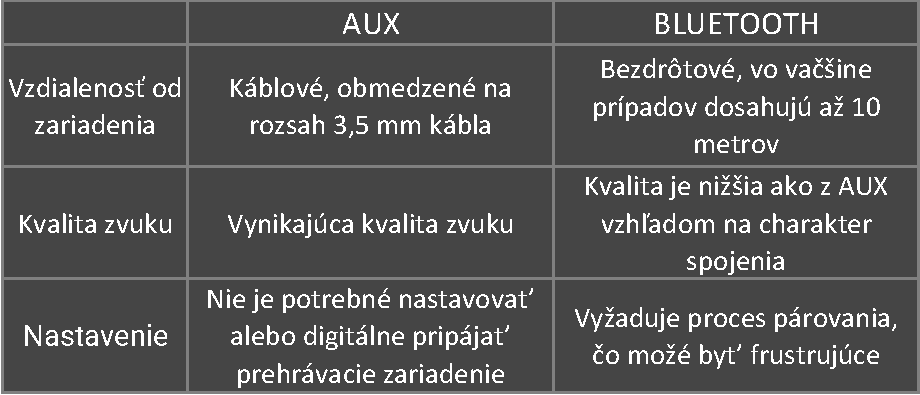
\includegraphics[scale=0.8]{AUXvsBluetooth.pdf}
\caption{Porovnanie AUX a Bluetooth.\cite{Laukkonen}}
\label{f:rozhod4}
\end{figure*}

\subsection{Pohodlie} \label{pohodlie} 

Pripojenie telefónu k reproduktorovému systému pomocou kábla Aux je jednoduché a možno aj rýchlejšie, ale prítomnosť kábla obmedzuje dosah medzi zariadením a jeho hostiteľom. Nie je potrebné digitálne nastavovať pripojenie Aux. Potrebujete iba konektor pre slúchadlá, ktorý vedie zo zdroja zvuku do vstupu Aux na reproduktore alebo prijímači. Na rozdiel od zvuku Bluetooth však pripojenia Aux vyžadujú fyzický kábel, ktorý sa môže stratiť alebo poškodiť.\cite{Laukkonen}

Bluetooth je bezdrôtový štandard, ktorý umožňuje väčšiu slobodu pohybu medzi zariadením a jeho hostiteľom. Väčšina pripojení je účinná na vzdialenosti do 33 stôp. Niektoré prípady priemyselného použitia dosahujú až 300 stôp alebo viac. Pre audio v aute umožňujú pripojenia Bluetooth hands-free ovládanie prostredníctvom virtuálnych asistentov, ako je Siri. To vám tiež umožňuje uskutočňovať hovory bez použitia rúk, čo nemôžete robiť s pripojením Aux.\cite{Laukkonen}

Pripojenie Bluetooth môže byť zložité. Ak chcete pripojiť telefón alebo zariadenie na prehrávanie médií k systému reproduktorov, musíte reproduktor umiestniť do režimu zisťovania a pomocou telefónu nájsť reproduktor. Tento proces nie je vždy taký jednoduchý, ako sa inzeruje. Ak sa dve zariadenia nespárujú, opakujte proces, kým nebude fungovať. Keďže softvér sa neustále aktualizuje, staré alebo zastarané zariadenia môžu predstavovať problém s pripojením. Niektoré párovania vyžadujú na dokončenie spojenia aj prístupový kód. To všetko môže spôsobiť, že proces prehrávania zvuku bude skôr problémom pri spúšťaní ako pomocou kábla Aux.\cite{Laukkonen}

\subsection{Kvalita zvuku} \label {kvalita}

Zvuk Bluetooth sa vo všeobecnosti považuje za horší ako väčšina káblových zvukových pripojení vrátane 3,5 mm pripojení Aux. Dôvodom je skutočnosť, že odosielanie zvuku cez bezdrôtové pripojenie Bluetooth zahŕňa kompresiu digitálneho zvuku na analógový signál na jednom konci a jeho dekomprimáciu na digitálny signál na strane druhej. Táto konverzia má za následok menšiu stratu vernosti zvuku.\cite{Laukkonen}

Hoci kvalita zvuku je teoreticky lepšia, Aux má nevýhody. Pretože ide o fyzické spojenie, Aux káble majú tendenciu sa časom opotrebovať. Opakované zasúvanie a odpájanie kábla môže pomaly erodovať kov a vytvárať zlé spojenia, ktoré skresľujú zvuk. Skraty v elektrickom toku tiež spôsobujú počuteľný šum. V prípade káblového pripojenia poskytujú digitálne pripojenia USB vo všeobecnosti lepšiu kvalitu zvuku, no nie každý si všimne rozdiel. \cite{Laukkonen}

Na špičkových zvukových systémoch sú tieto rozdiely jasné – či už cez Aux, Bluetooth alebo USB. Pripojenie Aux ako také poskytuje vyššiu kvalitu zvuku ako Bluetooth. Digitálne pripojenie (napríklad USB) poskytuje lepší zvuk. Rozdiely vo vernosti medzi jednotlivými zdrojmi musia byť porovnané s rozdielmi v pohodlí.\cite{Laukkonen}

\paragraph{Konečný verdikt} \label{verdikt} 

Je to preto, že Aux káble sú overené časom, že zostávajú také bežné. Prídavné káble nie sú bez nevýhod, ale jednoduché analógové pohodlie je jedným z dôvodov, prečo sú tieto káble obľúbené. To znamená, že Bluetooth dobieha.
Motiváciou Bluetooth bolo prísť s rýchlejšou, bezdrôtovou alternatívou k pripojeniu cez sériový port RS-232 pre osobné počítače v deväťdesiatych rokoch. Sériový port bol do konca tohto desaťročia z veľkej časti nahradený USB, ale Bluetooth si nakoniec našiel cestu do hlavného prúdu.
Bluetooth nie je štandardný modul pre 3,5 mm konektor pre slúchadlá. Každý štandard má svoje základné prípady použitia, ale ako sa médiá stávajú bezdrôtovejšími a digitálnymi, stáva sa aj prípad Bluetooth presvedčivejším.\cite{Laukkonen}

\section{Záver} \label{zaver} 

Každý kodek má svoje silné a slabé stránky, ale aký by mal byť kodek, aby bol absolútne obľúbený? Nižšie je uvedený zoznam, ktorý obsahuje hlavné charakteristiky, ktoré by mal predstavovať kodek budúcnosti. 

\begin {enumerate}
\item Bezpečnosť: Využíva všetky moderné bezpečnostné a kryptografické technológie.\cite{Stephens}
\item Otvorené: Open source a plne zdokumentované.\cite{Stephens}
\item Univerzálna podpora: Dá sa nahrávať a prehrávať bez potreby nového hardvéru alebo softvéru.\cite{Stephens}
\item Úplne bezstratové: ľahké a vysoko kvalitné.\cite{Stephens}
\item Viacnásobné použitie: Optimalizované pre hlasové a všeobecné použitie zvuku.\cite{Stephens}
\item Vysoké rozlíšenie: Podpora pre najvyššie možné rozlíšenie nahrávania.\cite{Stephens}
\end {enumerate}

Kodek, ktorý by zbieral všetky tieto parametre, zatiaľ neexistuje, no môžeme nájsť kodeky, ktoré sú v jednej kategórii lepšie a v inej horšie ako ostatné. Kodeky sa ako programy vyvíjajú veľmi rýchlo a preto môžeme čoskoro očakávať objavenie sa najnovších verzií, v ktorých sa bude zbierať stále viac ideálnych parametrov. Vzhľadom na to, že kodeky cez AUX a Bluetooth sa líšia svojou koncepciou, po chvíli si nebudeme môcť vybrať jednu kategóriu z týchto dvoch, takže ideálny kodek môžeme okamžite rozdeliť na dve miesta, jedno bude mať AUX a druhé Bluetooth. A obe tieto kategórie budú aktívne využívané, pretože možnosti AUX sú vhodnejšie pre domáce použitie a profesionálne účely a možnosti Bluetooth budú lepšie pre šport, autá a cestovanie.

\section{Reakcie na témy prednášok} \label{reakcie}

\paragraph{Bibliografia a citovanie v technickom texte} \label{bibliografia a citovanie}

"Pre každé tvrdenie, ktoré nie je vlastné tvrdenie autora alebo všeobecne známe, musí byť uvedený zdroj. Odkazov nikdy nie je veľa – len málo alebo primerane."\cite{bibliografia}.
Tieto dva hlavné princípy boli zdôraznené v prednáške o bibliografii. Zohľadnil som ich a snažil som sa, aby boli odkazy na zdroje čo najjasnejšie o tom, kde ich nájdete.

Súhlasím s tým, že citovanie zdrojov je neoddeliteľnou súčasťou písania článku a najdôležitejšou vlastnosťou citovania by mala byť ľahká identifikácia, o ktorom konkrétnom zdroji sa diskutuje a kde ho možno nájsť.

\paragraph {Vedecké publikovanie v informatike. Plagiátorstvo a ako sa mu vyhnúť.} \label{publikovanie a plagiatorstvo}

V tejto prednáške boli popísané hlavné zručnosti a výhody písania, sú nasledovné: poznanie, porozumenie, pochopiť problém, výskum, argumentácia, schopnosť písať, zlepšuje myslenie.\cite{plagiatorstvo}

Z tejto prednášky som sa naučil správny algoritmus na písanie esejí, dozvedel som sa aj viac o plagiátorstve a jeho dopade. Jasne sa písalo o patologickom kontexte napodobňovania, respektíve plagiátorstva.

"Preklad cudzieho textu je technicky to isté ako prevzatie. Prerozprávanie cudzieho textu bez uvedenia zdroja je tiež plagiát" \cite{plagiatorstvo} Preto je dôležité uviesť odkaz na zdroj, z ktorého čerpáme informácie.
Podporujem to, že hlavným spôsobom, ako vyriešiť problém s plagiátorstvom, je pokúsiť sa mu zabrániť všetkými možnými spôsobmi.\cite{plagiatorstvo}. Keďže aj neúmyselné plagiátorstvo je stále plagiátorstvo\cite{plagiatorstvo}, tak, ako odznelo na prednáške, treba sa zamerať na vlastný prínos. 
Myslím si, že rešpekt autorov je veľmi dôležitý, preto vždy budem necháť odkazy na zdroje iných tvorcov.

\paragraph{Grafické vyjadrenie informácií v informatike.} \label{Grafické vyjadrenie}

Raz vidieť je lepšie ako sto krát počuť. \footnote{Záturecký, A. P. Slovenské príslovia, porekadlá, úslovia a hádanky. Tatran. 2005}

Toto príslovie, ktoré bolo použité v prednáške\cite{Vizualizacia}, zdôrazňuje, že je veľmi dôležité si ho vizualizovať, aby bolo ľahšie pochopiť nové informácie. 
Pomocou určitých rôznych formulárov pri vytváraní sa môžete zamerať na jednotlivé časti kognitívne mapov, diagramov v tvare grafov atď. a zvýrazniť tak dôležité informácie.
Ešte lepším prístupom by bolo zobrazenie informácií z rôznych uhlov na označenie rôznych nuansov a vlastností konkrétnej témy.
Som si istý, že vizualizácia je jedným z najlepších spôsobov, ako prezentovať zložité fragmenty z článku.

\textit{...„Počujem a zabudnem. Vidím a pamätám. Robím a rozumiem.“ – Konfucius}\cite{Vizualizacia}. Tento jednoduchý citát vysvetľuje dôležitosť vizualizácie informácií pre čitateľa.


\bibliography{literatura}
\bibliographystyle{abbrv}
\end{document}
